\section{Machine Learning}
\subsection{Theory}

\subsubsection{Lecture 1}

Machine Learning differs from traditional programming, we want to model a function to predict data or patterns. Machine Learning has many applications in multiple fields. Since we are using data is important to notice that those can have biases like people. Some biases related to people can be confirmation, falalcy of centrality or survivorship.

\vspace{10pt}

ML as said has many applications, some can be:
\begin{enumerate}
    \item Image and object recognition
    \item Videogames
    \item Sound generation and recognition
    \item Art and style imitation
    \item Predictions
\end{enumerate}

\vspace{10pt}

Many algorithms exist for those tasks but all of them are made from three main components:
\begin{enumerate}
    \item \textbf{Representation} \ra Space of models
    \item \textbf{Evaluation} \ra How to assess which model is better for a certain task
    \item \textbf{Optimization} \ra How to improve the model
\end{enumerate}

Optimizing a model means finding the best parameters and hyperparameters, we can do it via:
\begin{itemize}
    \item Combinatorial optimization
    \item Convex optimization
    \item Constrained optimization
\end{itemize}

\vspace{10pt}

Different tasks require different kind of learning:

\begin{itemize}
    \item \textbf{Supervised/Inductive} \ra We have the labels of the training data
    \item \textbf{Unsupervised} \ra We don't have the labels in the training data
    \item \textbf{Semi-supervised} \ra Mix of the previous two
    \item \textbf{Reinforcement} \ra We want to maximize a reward function after performing some actions
\end{itemize}

More specifically we will study the first one

\vspace{10pt}

\textbf{Supervised} \ra We have many examples of data, we want to find the function that describes best their distribution. We can do classification, regression or estimating probabilities. The core idea is that we want to fit a curve that discriminates between classes or that fit at best a scatterplot. Since we are estimating we will have for sure a certain degree of errors, that is called the \textbf{bias}. Bias can also be positive if is used in a smart way, if we have knowledge about something we can use it to avoid useless steps.

\vspace{10pt}

As we know in the 1-D case a math function is on the form of 

\begin{equation}
    y = f(x)
\end{equation}

And if we open $f(x)$

\begin{equation}
    f(x) = ax + b
\end{equation}

This is the most basic linear case. We want to estimate the parameters a and b to fit the data in the best way. The core idea is to reduce as much uncertainty as possible.

\hrule

\subsubsection{Lecture 2}

Machine learning implies that the machine will learn something, there are different approaches for that. They can be applied to different tasks for better performances.

\begin{enumerate}
    \item \textbf{Symbolism} \ra Fill gaps in existing knowledge
    \item \textbf{Connectionism} \ra Emulate the brain
    \item \textbf{Evolutionary Computation} \ra Simulate evolution
    \item \textbf{Statistical Learning} \ra Reduce uncertainty
    \item \textbf{Analogy Modelling} \ra Check for similarities between old and new
\end{enumerate}

\begin{table}[h!]
\centering
\begin{tabular}{|l|l|l|}
\hline
\textbf{Tribe} & \textbf{Origins} & \textbf{Master Algorithm} \\ \hline
Symbolists & Logic, Philosophy & Inverse Deduction \\ \hline
Connectionists & Neuroscience & Backpropagation \\ \hline
Evolutionaries & Evolutionary Biology & Genetic Programming \\ \hline
Bayesians & Statistics, Probability & Inference \\ \hline
Analogizers & Psychology & Support Vector Machines (SVM) \\ \hline
\end{tabular}
\end{table}

\textbf{Symbolists}:
\begin{itemize}
    \item Logic programming
    \item Expert systems
    \item Decision trees
    \item Functional programming
\end{itemize}

\textbf{Connectionists}:
\begin{itemize}
    \item Perceptron
    \item MLP
    \item DNN
    \item Hopfield networks
    \item Boltzmann networks
\end{itemize}

\textbf{Evolutionary}:
\begin{itemize}
    \item Genetic algorithms
    \item Genetic programming
    \item Ant Colony optimization
    \item Particle Swarm optimization
\end{itemize}

\textbf{Bayesians}:
\begin{itemize}
    \item Bayesian classifiers
    \item Bayesian Belief networks
    \item Markov models
\end{itemize}

\textbf{Analogizers}:
\begin{itemize}
    \item KNN
    \item Self-organization
    \item SVM
\end{itemize}

If we cross together the tribes and the components seen in the previous class we can see that:

\begin{itemize}
    \item \textbf{Representation}
    \begin{itemize}
        \item Probabilistic Logic
        \item Each rule has a weight
    \end{itemize}
    \item \textbf{Evaluation}
    \begin{itemize}
        \item Posterior probability
        \item User defined objective function
    \end{itemize}
    \item \textbf{Optimization}
    \begin{itemize}
        \item Genetic programming
        \item Backpropagation
    \end{itemize}
\end{itemize}


\subsubsection{Lecture 3}

The most important part of a machine learning model is the dataset, sometimes the data aren't good enough on their own so we must account for that. Some ways are

\begin{itemize}
    \item \textbf{Feature extraction and engineering} \ra extract something from simpler features
    \item \textbf{Feature transformation} \ra modify the features to make them more useful for the model
    \item \textbf{Feature selection} \ra use the most relevant features
\end{itemize}

In this course we will see mainly the third point. When we do \textbf{Feature selection} we aim to reduce the number of inputs variables to a subset that can be equally useful. Simpler models are easier to interpret, the training time is reduced, generalization is enhanced and we remove redundant variables.

\vspace{10pt}

Feature selection is done via 3 main methods:
\begin{itemize}
    \item \textbf{Filter methods} \ra Statistical methods to evaluate the importance of the features, like correlation
    \item \textbf{Wrapper methods} \ra We train a model with subsets of features until we find the best one
    \item \textbf{Embedded methods} \ra During the training of our model the importance of the features is assessed. 
\end{itemize}

\textbf{Filter methods}:
\begin{itemize}
    \item Pearson correlation coefficient
    \item Spearman rank coefficient
    \item ANOVA correlation coefficient
    \item Kendall rank coefficient
    \item Chi-Squared test
    \item Mutual information
\end{itemize}

\vspace{10pt}

Pearson Correlation coefficient, it measures linear correlation:
\begin{equation*}
    \rho_{X,Y} = \frac{\text{cov(X,Y)}}{\sigma_X \sigma_Y}
\end{equation*}

For m samples

\begin{equation*}
r = \frac{\sum_{i=1}^{m} (x_i - \bar{x})(y_i - \bar{y})}
{\sqrt{\sum_{i=1}^{m} (x_i - \bar{x})^2} \; \sqrt{\sum_{i=1}^{m} (y_i - \bar{y})^2}}
\end{equation*}

Spearman rank correlation coefficient, it asses how well the relationship between two variables can be described by a monotonic function

\begin{equation*}
    r_s = \rho_{rg_x,rg_y}= \frac{cov(rg_x,rg_y}{\sigma_{rg_x}\sigma_{rg_y}}
\end{equation*}

\vspace{10pt}

We shouldn't always discard variables with a small score. It depends by case to case

\vspace{10pt}

We can also use \textbf{Mutual information}, this can help finding non-linear dependencies but is harder to estimate than pure correlation.

\vspace{10pt}

Mutual information (continuous and discrete), for non linear and non monotonic relationships

% Caso continuo
\begin{equation*}
I(X_i; y) = \int \int p(x_i, y) \, \log \frac{p(x_i, y)}{p(x_i)\, p(y)} \, dx \, dy
\end{equation*}

% Caso discreto
\begin{equation*}
I(X_i; Y) = \sum_{x_i} \sum_{y} P(X = x_i, Y = y) \, \log \frac{P(X = x_i, Y = y)}{P(X = x_i) \, P(Y = y)}
\end{equation*}

The problem is that mutual information can be inconvenient for feature ranking. To solve the associated problems we can use the \textbf{Maximal information coefficient} that transforms the previous and binds it in [0;1]. We obtain the percent of a variable Y that can be explained by a variable x

\begin{equation*}
\text{MIC}(X, Y) = \max \{\frac{I(x, y)}{\log_2 \min\{ n_x, n_y \}}\}
\end{equation*}

\vspace{10pt}

\textbf{Wrapper methods}

We consider certain subsets of our features, at each iteration we try to find the best combination of those. We can vary which and how many features to consider. The selection process involves evaluate the subsets using a predictive model and using the subset with the best performance.

\vspace{10pt}

The search process can use different strategies:
\begin{itemize}
    \item Methodical
    \item Stochastic
    \item Heuristics
\end{itemize}

\vspace{10pt}

One of the most used is RFE
\begin{enumerate}
    \item The model is fitted on all the predictors
    \item Each predictor is ranked using it's importance to the model
    \item We choose the n top ranked predictors
    \item We find the best number n with the best n features
\end{enumerate}

RFE can encounter problems if it overfit on uninformative features.

\vspace{10pt}

Our training set is used for selecting predictors, fitting the model and evaluating the performance.

To improve RFE we can add \textbf{Cross-validation}

\vspace{10pt}

\textbf{Embedded methods}

This last kind of methods consists in regularizing the model while it's been created. The process consists in adding constraints into the optimization and adding a bias toward lower complexity, so reducing the number of coefficients

\vspace{10pt}

We have two main regularization algorithms:
\begin{enumerate}
    \item Ridge, or L2
    \item Lasso or L1
\end{enumerate}

\vspace{10pt}

Ridge Regression tries to minimize the sum of squared residuals and the slope of the line. This can cause many lower coefficients and can solve for parameters where we do not enough data samples.

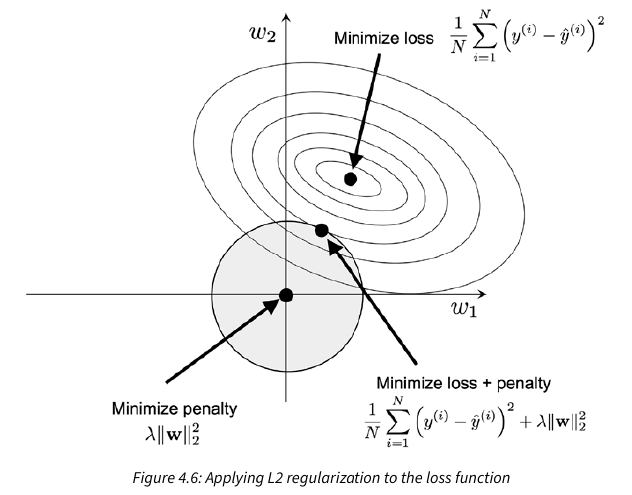
\includegraphics{L2.png}

\vspace{10pt}

Lasso Regression on the other hand tries to minimize the magnitudes. It can lead to many zero values in our coefficients set

%\begin{tikzpicture}
%\node[inner sep=0pt] at (0,0) {\pgfimage[width=10cm]{Courses/images/L1.png}};
%\end{tikzpicture}

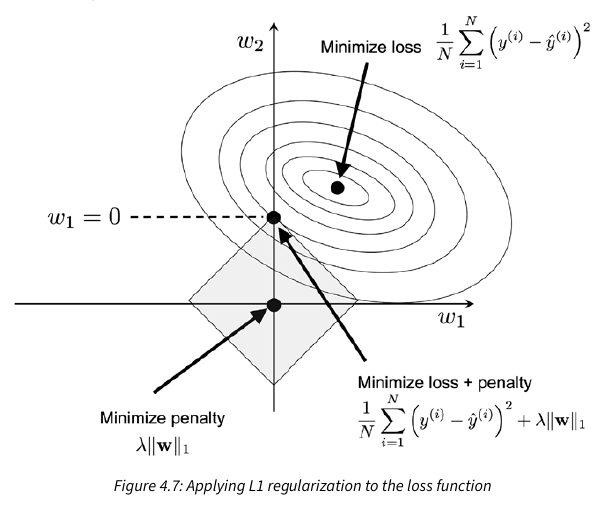
\includegraphics{L1.png}





\hrule



\subsubsection{Lecture 4}

Today we look at our first algorithms, we start with \textbf{Linear Regression}.

\vspace{10pt}

We want to find a relationship between independent variables and the dependent one. The objective is to make predictions based on the past observations.

\vspace{10pt}

As we know one kind of task for ML models is regression, we want to predict a continuous values. One way is using Linear Regression.

The steps are:
\begin{enumerate}
    \item Use least-squares to fit a line on the data
    \item Calculate the $R^2$
    \item Calculate the p-value for $R^2$
\end{enumerate}

A regression model can be simple or multiple

\begin{equation}
    Y = \beta_0 + \beta_1X_1+ \beta_2X_2+...+\beta_nX_n+\varepsilon
\end{equation}

Where:
\begin{itemize}
    \item Y \ra Model/output
    \item $\beta_0$ \ra Intercept
    \item $\beta_n$ \ra Parameters
    \item $X_n$ \ra Inputs
    \item $\varepsilon$ \ra Residuals
\end{itemize}

\vspace{10pt}

For the simple model we only use the first 2 $\beta$ and the first X

We want to minimize the squared sum of the residuals, this will give us a good model. Since this is a minimization problem on both the parameters we differentiate them getting the following formulas (notes that those are estimations)

\begin{equation}
    \hat{\beta_1} = \frac{\Sigma(X_i-\bar{X})(Y_i-\bar{Y})}{\Sigma(X_i-\bar{X})^2}
\end{equation}

\begin{equation}
    \hat{\beta_0} = \hat{Y} - \hat{\beta_1}\bar{X}
\end{equation}

\vspace{10pt}

As said these are estimations, so we want to evaluate how good they are.

Usually we use $R^2$, it explains how much variation in the output can be explained differently from using just the mean.

\begin{equation}
    R^2 = \frac{SS(mean)- SS(fit)}{SS(mean)}
\end{equation}

Where

\begin{itemize}
    \item SS(mean) or SST \ra $\Sigma(y_i-\bar{y})^2$
    \item SS(fit) or SSE = \ra $\Sigma(y_i-\hat{y_i})^2$
\end{itemize}

\vspace{10pt}

We can also do

\begin{equation}
    R^2=\frac{\text{Var(mean) - Var(fit)}}{\text{Var(mean)}}
\end{equation}

Where

\begin{itemize}
    \item Var(mean) = $\frac{\Sigma(y_i-\bar{y})^2}{n}$ = $\frac{SS(mean)}{n}$
    \item Var(fit) = $\frac{\Sigma(y_i-\hat{y}_i)^2}{n}$ = $\frac{SS(fit)}{n}$
\end{itemize}

\vspace{10pt}

Since bigger models with more features will explain more variability we can use the adjusted $R^2$, it will penalize models with a lot of independent variables

\begin{equation}
    \text{Adjusted }R^2 = 1-\frac{(1-R^2)(N-1)}{N-p-1}
\end{equation}

Where
\begin{itemize}
    \item $R^2$ \ra Current $R^2$
    \item N \ra Samples
    \item p \ra Number of independent variables
\end{itemize}

\vspace{10pt}

After that we can check the p-value for each independent variable to check it's statistical relevance, low p-value means high probability that the variable is useful.

\vspace{10pt}

Another model that we have to look at is \textbf{Logistic Regression}, despite the name is a classifier and not a regressor. We want to make a binary classification (1 or 0) based on our data. Differently from the Linear regression loss function (SSE) here we use MLE (Maximum Likelihood Estimation) to maximize the probability of being right.

\vspace{10pt}

Usually our decision is like this

\begin{equation}
    \begin{cases}
        \text{1 \hspace{10pt} if True} \\
        \text{0 \hspace{10pt} if False}
    \end{cases}
\end{equation}

In such cases we can't easily (or we straight up can't) linearly separate those examples, the we need a non linear discriminator with an output between 0 and 1. We want to model the probabilities of being of either class. The function used is a Sigmoid.

\begin{equation}
    p = \frac{1}{1 + e^{-(\beta_0 +\beta_1x)}}
\end{equation}

As said we use MLE to estimate the parameters of the function. Basically we maximise the 
probability of observing the sample.

\vspace{10pt}

Since we want to get a probability between 0 and 1 we have to follow some passages.
\begin{itemize}
    \item We start from the probability \(p = P(Y=1 \mid X)\).
    \item We convert it into \textbf{odds}: \(\dfrac{p}{1-p}\), which range from \(0\) to \(+\infty\).
    \item We take the \textbf{log} of the odds (logit): \(\log\left(\dfrac{p}{1-p}\right)\), which can take any real value \((-\infty, +\infty)\).
    \item We model the log-odds with a \textbf{linear function of the inputs}:  
    \[
    \log\left(\dfrac{p}{1-p}\right) = \beta_0 + \beta_1 x_1 + \dots + \beta_k x_k
    \]
    \item We estimate the parameters \(\beta_0, \beta_1, \dots, \beta_k\) using \textbf{Maximum Likelihood}:  
    each observed \(y_i\) contributes a probability  
    \[
    p_i^{\,y_i} (1 - p_i)^{\,1 - y_i}
    \]
    and we choose the parameters that maximize the likelihood of all observations.
    \item Once the parameters are learned, we plug the linear combination back and convert it to a probability:
    \[
    p = \frac{1}{1 + e^{-(\beta_0 + \beta_1 x_1 + \dots + \beta_k x_k)}}
    \]
    \item This final expression is the \textbf{sigmoid (logistic) function}, which always returns a value between 0 and 1.
\end{itemize}

\vspace{10pt}

To estimate the parameters and how to interpret them:

\begin{itemize}
    \item Parameters are chosen to maximize the likelihood of observing the sample.
    \item Unlike linear regression, there are no closed-form formulas.
    \item We maximize the \textbf{log-likelihood} numerically.
    \item ML estimates are obtained iteratively until the log-likelihood stabilizes.
    \item Predicted log-odds:
    \[
        \hat{y}_i = \hat{\beta}_0 + \hat{\beta}_1 x_{1i} + \dots + \hat{\beta}_k x_{ki}
    \]
    \item Estimated probability:
    \[
        \hat{P}(Y_i=1|X_i) = \frac{e^{\hat{y}_i}}{1+e^{\hat{y}_i}}
    \]
    \item Sign of \(\hat{\beta}_k\) indicates direction of curve:
    \begin{itemize}
        \item \(\hat{\beta}_k > 0\) : probability increases with \(x_k\)
        \item \(\hat{\beta}_k < 0\) : probability decreases with \(x_k\)
    \end{itemize}
    \item Rate of change increases with magnitude of \(\hat{\beta}_k\)
    \item Example: \(\hat{malign}_i = -7.7836 + 0.6683 \cdot thickness + 0.5540 \cdot size + 0.6807 \cdot shape\)
    \begin{itemize}
        \item thickness=5, size=2, shape=2 \(\Rightarrow \hat{P} \approx 0.12\)
        \item thickness=10, size=8, shape=9 \(\Rightarrow \hat{P} \approx 0.999\)
    \end{itemize}
\end{itemize}



\vspace{10pt}

\hrule

\vspace{10pt}

\subsubsection{Lecture 5}

Today we see model selection with Carina Albuquerque (breaking bad mentioned).

\vspace{10pt}

We want to find the best model from a set of possible ones. Either comparing different models or different hyperparameters and the same model.

\vspace{10pt}

We want to reduce overfitting, emphasize understanding vs memorizing the data.

\vspace{10pt}

The Model selection follows these steps

\begin{enumerate}
    \item Split in Train (training the parameters, 70\%), Validation (best model and parameters, 15\%), Test (test the performance, 15\%)

    \item Choose the metric

    \item Choose the eval method

    \item Run the models

    \item Compare metrics

    \item Pick the model
    
\end{enumerate}


\vspace{10pt}

To avoid overfitting we should minimize the Validation error and the Training error. When both are minimized we find the best complexity for our model. The opposite of overfitting is called underfitting.

\vspace{10pt}

If the dataset is imbalanced we apply stratification. Or use SMOTE.

\vspace{10pt}

Use k-fold CrossValidation to get the more realistic performance and improve training, usually 10 folds. We can also have Leave-One-out cross val.

\vspace{10pt}

Usually the best model is the one with better performance. We have a trade off between simpler models and their accuracy. Interpretable models are usually the simple ones. This is also true for time needed for the training.


\vspace{10pt}

Test set and hold out \ra Big data
Cross-val \ra Middle data



\textbf{Model Assessment} is a way to quantify the strength of the model.

The usual metrics are

\begin{itemize}
    \item 
\end{itemize}










\subsection{Brief recap of models and other useful things}

\subsubsection{Lecture 1}

\begin{itemize}
    \item \textbf{Training example:} A pair $(x, f(x))$.
    \item \textbf{Target function:} The true function $f(x)$ that we want to estimate.
    \item \textbf{Hypothesis:} A proposed function $h$, believed to be similar to $f$; the output of the learning algorithm.
    \item \textbf{Concept:} Boolean function that describes the instances of the dataset.
          \begin{itemize}
              \item $f(x) = 1 \;\Rightarrow$ positive example
              \item $f(x) = 0 \;\Rightarrow$ negative example 
          \end{itemize}
    \item \textbf{Classifier:} A discrete-valued function produced by the learning algorithm.  
          The possible values of $f \in \{1,2,\dots,K\}$ are the \emph{classes} or \emph{class labels}.  
          (In most algorithms the classifier actually returns a real-valued function that must be interpreted).
    \item \textbf{Hypothesis space:} The space of all hypotheses that can, in principle, be produced by the learning algorithm.
    \item \textbf{Version space:} The subset of the hypothesis space that has not yet been ruled out by the training examples.
\end{itemize}


\subsubsection{Lecture 2}
\subsubsection{Lecture 3}
\subsubsection{Lecture 4}
% \subsubsection{Lecture 5}

\subsection{Things seen at the practical}
